\documentclass{sjtuarticle}
\subject{区块链技术}
\title{第七次作业}
\author{李子龙\\123033910195}
\usepackage{tikz}
\usetikzlibrary{arrows.meta}
\usepackage{ntheorem}
\usepackage[colorlinks]{hyperref}

\def\pk#1{\mathit{PK}_{#1}}
\def\pki#1#2{\mathit{PK}_{#1#2}^\prime}

\begin{document}
\maketitle

服务提供商规定一些面值的比特币交易,比如:100, 50, 10, 5, 1, 0.5, 0.1,由于服务提供商会知道公钥 $\mathit{PK}_i$ 与用户 $i$ 的对应关系,根据用户需要洗币的金额 $v$,按照找零算法(先换大面值,再换小面值)计算需要的接收公钥数 $n_i$,服务提供商会要求用户提供对应数目的接收公钥 $\mathit{PK}_{ij}^\prime (j=1,\cdots,n)$。服务提供商将会给用户提供服务的接收公钥地址 $\mathit{PK}_S$。

用户与服务器交换完公钥地址信息后,用户以公钥 $\mathit{PK}_i$ 向服务器地址 $\mathit{PK}_S$ 发送 $v$ 比特币,服务器在接收到其他用户足够的金额的比特币后,会用其他用户发送给服务器产生的 UTXO 发送给用户提供的接收公钥地址 $\mathit{PK}_{ij}^\prime$,这些交易之间会有相对随机的间隔时间,这样就达到了洗币的目的。服务提供者可能会收取服务费。

为了保障隐私,服务者应该保证公钥与用户的对应信息不被泄漏,即 $\pk{i}$ 与 $\pki{i}{j}$ 的对应关系。并且服务者需要保证不会克扣除服务费外的其他比特币。

为了简化讨论的情形,假设服务提供者不收取服务费。这里还假设可以有除了 A,B,C 外的其他用户,比如 D,E,F 等。因为:
\begin{itemize}
    \item 服务提供者需要足够多的用户才可以为用户提供足够好的隐私性,以更好地混合,提供更有隐私的服务;
    \item 使用找零算法可能会产生无法完全匹配的情况,但是好处就是这个算法是确定性的,在用户提交需求时就可以按照预先设定的面额得知需要多少个接收公钥地址,而不是取决于服务器的运营情况;
    \item 不需要中间服务者的情况可以考虑 Coin-Join,一般 Coin-Join 都会基本让交换的币值相等。如果服务器决定用相同的面值,那么该面值会不可避免地足够小,从而产生过多的交易,而大幅降低服务效率。
\end{itemize}

回到本题的具体情景,根据找零算法,分拆用户提供的金额:
\begin{align*}
    A&: 115 = 100 + 10 + 5 \\
    B&: 120 = 100 + 10 + 10 \\
    C&: 12 = 10 + 1 + 1
\end{align*}

这样,A、B、C都应该各自分别提供3个接收公钥地址 $\mathit{PK}_{Aj}^\prime (j=1,2,3)$、$\mathit{PK}_{Bj}^\prime (j=1,2,3)$、$\mathit{PK}_{Cj}^\prime (j=1,2,3)$。假设服务器又接收到了 D 的 5 比特币,E 的 1 比特币,F 的 1 比特币,他们也都提供了对应的接收公钥地址 $\mathit{PK}_{D1}^\prime, \mathit{PK}_{E1}^\prime, \mathit{PK}_{F1}^\prime$。

交易最终流向如下:
% \begin{align*}
%     (\pk{A},115)\rightarrow(\pk{S},115)\rightarrow(\pki{B}{1},100)+[(\pk{S},15)\rightarrow(\pki{B}{2},10)+[(\pk{S},5)\rightarrow(\pki{D}{1},5)]]\\
%     (\pk{B},120)\rightarrow(\pk{S},120)\rightarrow(\pki{A},100)+(\pki{B}{3},10)+(\pki{C}{1},10)\\
%     (\pk{C},12)\rightarrow
% \end{align*}
\begin{align*}
    A&: 115 = 100(\pki{B}{1}) + 10(\pki{B}{2}) + 5(\pki{D}{1}) \\
    B&: 120 = 100(\pki{A}{1}) + 10(\pki{A}{2}) + 10(\pki{C}{1}) \\
    C&: 12 = 10(\pki{B}{3}) + 1(\pki{E}{1}) + 1(\pki{F}{1})\\
    D&: 5 = 5(\pki{A}{3}) \\
    E&: 1 = 1(\pki{C}{2}) \\
    F&: 1 = 1(\pki{C}{3})
\end{align*}

具体的交易图如图 \ref{fig:tx} 所示,其中 $(\pk{i},v)$ 表示一“枚”比特币,即公钥地址 $\pk{i}$ 上的 $v$ 金额的 UTXO。交易 $tx$ 按时间顺序编号,实际上只要保证交易依赖关系树后级的交易在得知地址信息的情况下晚于前级的交易即可。
\begin{figure}[h]
    \centering
    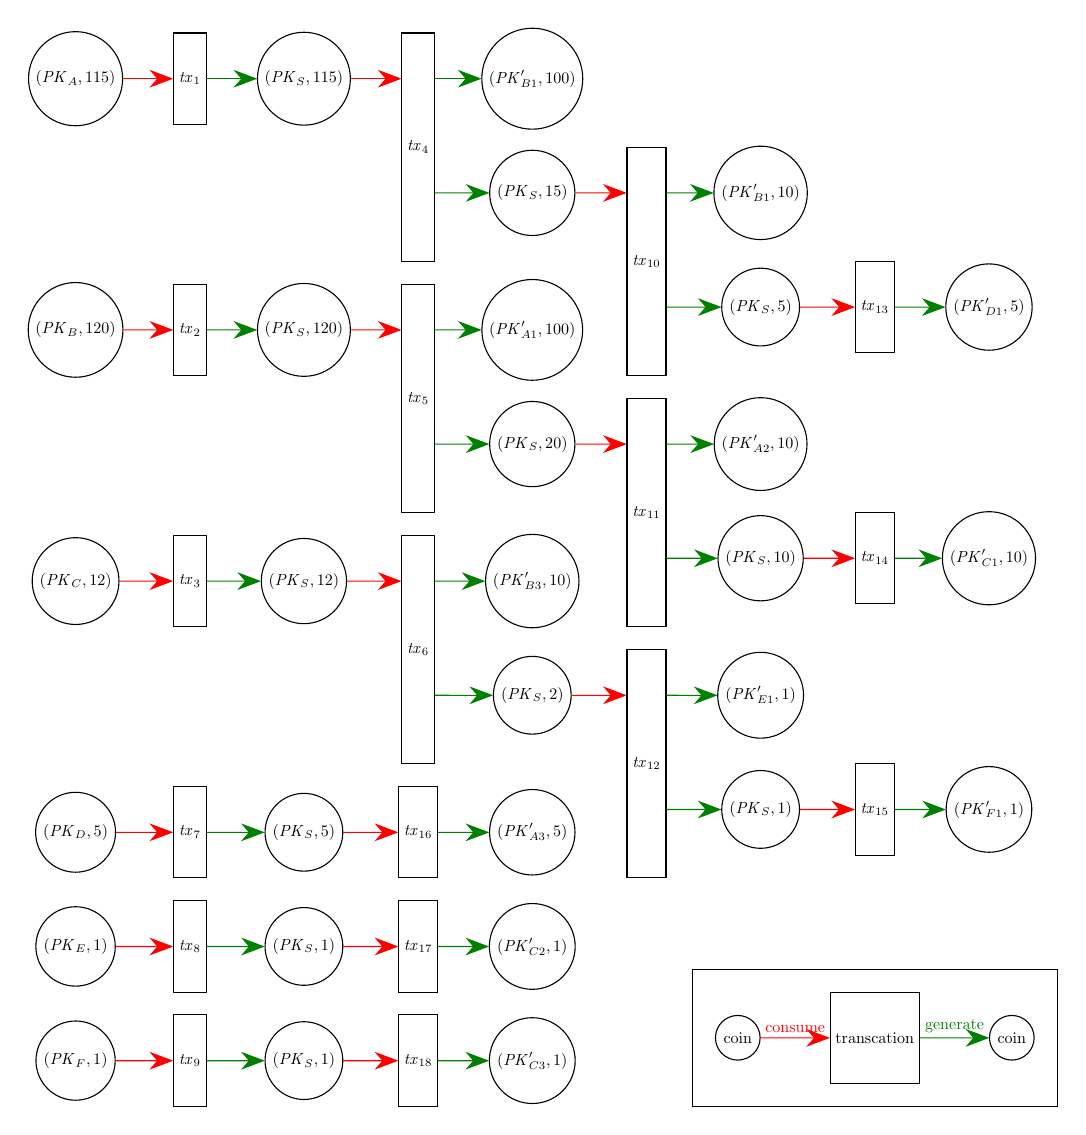
\begin{tikzpicture}[scale=0.58,every node/.style={scale=0.58}]
\def\pkv#1#2{$(\mathit{PK}_{#1},#2)$}
\def\pkiv#1#2#3{$(\mathit{PK}_{#1#2}^\prime,#3)$}
\def\tx#1{$\mathit{tx}_{#1}$}
\tikzstyle{coin}=[draw,circle];
\tikzstyle{tx0}=[draw,text centered,minimum height=2cm];
\tikzstyle{tx1}=[draw,text centered,minimum height=5cm];
\tikzstyle{con}=[-{Stealth[length=3mm]},red];
\tikzstyle{gen}=[-{Stealth[length=3mm]},green!50!black];

\node [coin] (v1) at (0,0) {\pkv{A}{115}};
\node [tx0] (v2) at (2.5,0) {\tx{1}};
\draw [con] (v1) -- (v1 -| v2.west);

\node [coin] (v3) at (5,0) {\pkv{S}{115}};
\draw [gen] (v2.east |- v3) -- (v3);
\node [tx1] (v4) at (7.5,-1.5) {\tx{4}};

\draw [con]  (v3) -- (v3 -| v4.west);
\node [coin] (v5) at (10,0) {\pkiv{B}{1}{100}};
\draw [gen] (v4.east |- v5) -- (v5);
\node [coin] (v6) at (10,-2.5) {\pkv{S}{15}};
\draw [gen] (v4.east |- v6) -- (v6);


\node [tx1] (v24) at (12.5,-4) {\tx{10}};
\node [coin] (v25) at (15,-2.5) {\pkiv{B}{1}{10}};
\node [coin] (v26) at (15,-5) {\pkv{S}{5}};
\draw [con] (v6) -- (v6 -| v24.west);
\draw [gen] (v24.east |- v25) -- (v25);
\draw [gen] (v24.east |- v26) -- (v26);
\node [tx0] (v27) at (17.5,-5) {\tx{13}};
\node [coin] (v28) at (20,-5) {\pkiv{D}{1}{5}};
\draw [con] (v26) edge (v27);
\draw [gen] (v27) edge (v28);

%%

\node [coin] (v7) at (0,-5.5) {\pkv{B}{120}};
\node [tx0] (v8) at (2.5,-5.5) {\tx{2}};
\draw [con] (v7) -- (v7 -| v8.west);

\node [coin] (v9) at (5,-5.5) {\pkv{S}{120}};
\draw [gen] (v8.east |- v9) -- (v9);
\node [tx1] (v10) at (7.5,-7) {\tx{5}};

\draw [con]  (v9) -- (v9 -| v10.west);
\node [coin] (v11) at (10,-5.5) {\pkiv{A}{1}{100}};
\draw [gen] (v10.east |- v11) -- (v11);
\node [coin] (v12) at (10,-8) {\pkv{S}{20}};
\draw [gen] (v10.east |- v12) -- (v12);

\node [tx1] (v24) at (12.5,-9.5) {\tx{11}};
\node [coin] (v25) at (15,-8) {\pkiv{A}{2}{10}};
\node [coin] (v26) at (15,-10.5) {\pkv{S}{10}};
\draw [con] (v12) -- (v12 -| v24.west);
\draw [gen] (v24.east |- v25) -- (v25);
\draw [gen] (v24.east |- v26) -- (v26);
\node [tx0] (v27) at (17.5,-10.5) {\tx{14}};
\node [coin] (v28) at (20,-10.5) {\pkiv{C}{1}{10}};
\draw [con] (v26) edge (v27);
\draw [gen] (v27) edge (v28);

%%

\node [coin] (v13) at (0,-11) {\pkv{C}{12}};
\node [tx0] (v14) at (2.5,-11) {\tx{3}};
\draw [con] (v13) -- (v13 -| v14.west);

\node [coin] (v15) at (5,-11) {\pkv{S}{12}};
\draw [gen] (v14.east |- v15) -- (v15);
\node [tx1] (v16) at (7.5,-12.5) {\tx{6}};

\draw [con]  (v15) -- (v15 -| v16.west);
\node [coin] (v17) at (10,-11) {\pkiv{B}{3}{10}};
\draw [gen] (v16.east |- v17) -- (v17);
\node [coin] (v18) at (10,-13.5) {\pkv{S}{2}};
\draw [gen] (v16.east |- v18) -- (v18);


\node [tx1] (v24) at (12.5,-15) {\tx{12}};
\node [coin] (v25) at (15,-13.5) {\pkiv{E}{1}{1}};
\node [coin] (v26) at (15,-16) {\pkv{S}{1}};
\draw [con] (v18) -- (v18 -| v24.west);
\draw [gen] (v24.east |- v25) -- (v25);
\draw [gen] (v24.east |- v26) -- (v26);
\node [tx0] (v27) at (17.5,-16) {\tx{15}};
\node [coin] (v28) at (20,-16) {\pkiv{F}{1}{1}};
\draw [con] (v26) edge (v27);
\draw [gen] (v27) edge (v28);


%%

\node [coin] (v19) at (0,-16.5) {\pkv{D}{5}};
\node [tx0] (v20) at (2.5,-16.5) {\tx{7}};
\draw [con] (v19) -- (v20);
\node [coin] (v21) at (5,-16.5) {\pkv{S}{5}};
\draw [gen] (v20) edge (v21);
\node [tx0] (v22) at (7.5,-16.5) {\tx{16}};
\draw [con] (v21) -- (v22);
\node [coin] (v23) at (10,-16.5) {\pkiv{A}{3}{5}};
\draw [gen] (v22) edge (v23);


\node [coin] (v19) at (0,-19) {\pkv{E}{1}};
\node [tx0] (v20) at (2.5,-19) {\tx{8}};
\draw [con] (v19) -- (v20);
\node [coin] (v21) at (5,-19) {\pkv{S}{1}};
\draw [gen] (v20) edge (v21);
\node [tx0] (v22) at (7.5,-19) {\tx{17}};
\draw [con] (v21) -- (v22);
\node [coin] (v23) at (10,-19) {\pkiv{C}{2}{1}};
\draw [gen] (v22) edge (v23);


\node [coin] (v19) at (0,-21.5) {\pkv{F}{1}};
\node [tx0] (v20) at (2.5,-21.5) {\tx{9}};
\draw [con] (v19) -- (v20);
\node [coin] (v21) at (5,-21.5) {\pkv{S}{1}};
\draw [gen] (v20) edge (v21);
\node [tx0] (v22) at (7.5,-21.5) {\tx{18}};
\draw [con] (v21) -- (v22);
\node [coin] (v23) at (10,-21.5) {\pkiv{C}{3}{1}};
\draw [gen] (v22) edge (v23);

%%

\node [coin] (v29) at (14.5,-21) {coin};
\node [tx0] (v30) at (17.5,-21) {transcation};
\node [coin] (v31) at (20.5,-21) {coin};
\draw [con] (v29) edge node[above,red] {consume} (v30);
\draw [gen] (v30) edge node[above,green!50!black] {generate} (v31);
\draw  (13.5,-19.5) rectangle (21.5,-22.5);
\end{tikzpicture}
    \caption{交易图}
    \label{fig:tx}
\end{figure}


% A: 115 = 100(B) + 10(B) + 1(C) + 1(C) + 1(B) + 1(B) + 1(B)
% B: 120 = 100(A) + 10(C) + 10
% C: 12 = 10(B) + 1(A) + 1(A)

% 100
% 50
% 20
% 10
% 5
% 1
% 0.5
% 0.1

% UTXO1->Server->PK2

% https://en.bitcoin.it/wiki/Privacy#Centralized_mixers
%
% There are several downsides to this. The mixer it must be trusted to keep secret the linkage between the incoming and outgoing transactions. Also the mixer must be trusted not to steal coins. This risk of stealing creates reputation effects; older and more established mixers will have a better reputation and will be able to charge fees far above the marginal cost of mixing coins. Also as there is no way to sell reputation, the ecosystem of mixers will be filled with occasional exit scams.


\end{document}